% (c) 2013 Claudio Carboncini - claudio.carboncini@gmail.com
% (c) 2017 Daniele Zambelli - daniele.zambelli@gmail.com
% 
% Tutti i grafici per il capitolo relativo alla probabilità
%

\newcommand{\unioneeventi}{%
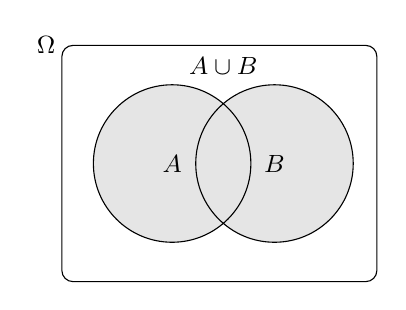
\begin{tikzpicture}[filled/.style={fill=circle area, draw=black, 
thin},x=10mm,y=10mm,font=\small]

\def\firstcircle{(1.4,1.5) circle (1cm)}
\def\secondcircle{(2.7,1.5) circle (1cm)}

\definecolor{circle area}{gray}{.9}

 \draw[filled] \firstcircle node {$A$}
                  \secondcircle node {$B$};
 \node[anchor=south] at (current bounding box.north) {$A \cup B$};
\draw[rounded corners] (0,0) rectangle (4,3) (-.2,3) node {$\Omega$} ;
\end{tikzpicture}
}

\newcommand{\implicazioneeventi}{%
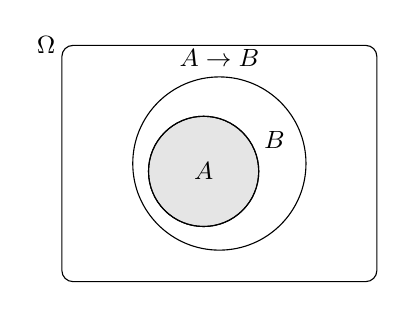
\begin{tikzpicture}[filled/.style={fill=circle area, draw=black, 
thin},x=10mm,y=10mm,font=\small]
\def\firstcircle{(2,1.5) circle (1.1cm)}
\def\secondcircle{(1.8,1.4) circle (.7cm)}

\definecolor{circle edge}{gray}{0.9}
\definecolor{circle area}{gray}{0.9}
    \begin{scope}
        \clip \firstcircle;
        \fill[filled] \secondcircle;
    \end{scope}
    \draw\firstcircle;
    \node[]  at (2.7,1.8) {$B$}; 
    \draw \secondcircle node {$A$};
    \node[anchor=south] at (current bounding box.north) {$A \to B$};
\draw[rounded corners] (0,0) rectangle (4,3) (-.2,3) node {$\Omega$} ;
\end{tikzpicture}
}

\newcommand{\eventiincompatibili}{%
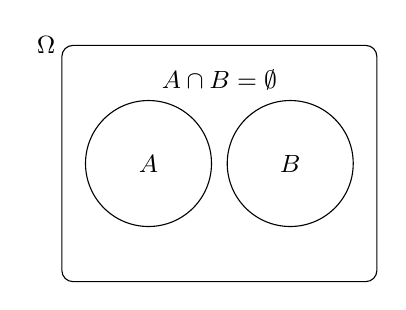
\begin{tikzpicture}[filled/.style={fill=circle area, draw=circle edge, 
thick},x=10mm,y=10mm,font=\small]
\def\firstcircle{(1.1,1.5) circle (.8cm)}
\def\secondcircle{(2.9,1.5) circle (.8cm)}

\definecolor{circle edge}{gray}{0.8}
\definecolor{circle area}{gray}{0.8}
    \begin{scope}
        \clip \firstcircle;
        \fill[filled] \secondcircle;
    \end{scope}
    \draw\firstcircle node {$A$};
    \draw \secondcircle node {$B$};
    \node[anchor=south] at (current bounding box.north) {$A \cap B=\emptyset$};
\draw[rounded corners] (0,0) rectangle (4,3) (-.2,3) node {$\Omega$} ;
\end{tikzpicture}
}

\newcommand{\eventiesaustivi}{% 
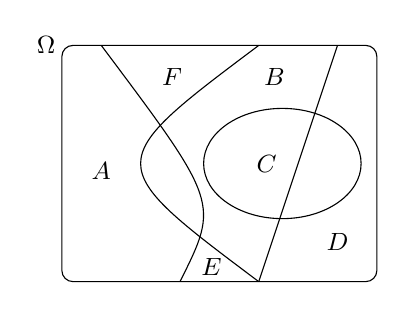
\begin{tikzpicture}[x=10mm,y=10mm,font=\small]
\draw[rounded corners] (0,0) rectangle (4,3) (-.2,3) node {$\Omega$} ;
\draw (.5, 3) .. controls(2,1) .. (1.5, 0);
\node at (.5,1.4) {$A$};
\draw (2.5, 3) .. controls(.5,1.5) .. (2.5, 0);
\node at (2.7,2.6) {$B$};
\draw (2.8,1.5) ellipse (1 and .7);
\node at (2.6,1.5) {$C$};
\draw (3.5,3) -- (2.5,0);
\node at (3.5,.5) {$D$};
\node at (1.9,.18) {$E$};
\node at (1.4,2.6) {$F$};
\end{tikzpicture}
}

\newcommand{\partizioneeventi}{
\begin{tikzpicture}[x=10mm,y=10mm,font=\small]
\draw[rounded corners] (0,0) rectangle (4,3) (-.2,3) node {$\Omega$} ;
%insiemi F ed E
\draw [name path=curva1] (.5, 3) .. controls(2,1) .. (1.5, 0);
\draw [color=white, name path=curva2] (2.5, 3) .. controls(.5,1.5) .. (2.5, 0);
\coordinate [name intersections={of=curva1 and curva2, by={a,b}}];
\draw (a) -- (2.5,3);
\draw (b) -- (2.5,0);
%insiemi B ed D
\draw [name path=elipse1] (2.8,1.5) ellipse (1 and .7);
\draw [color=white, name path=linea1] (3.5,3) -- (2.5,0);
\coordinate [name intersections={of=elipse1 and linea1, by={c,d}}];
\draw (c) -- (3.5,3);
\draw (d) -- (2.5,0);

\node at (.5,1.4) {$A$};
\node at (2.7,2.6) {$B_1$};
\node at (2.6,1.5) {$C$};
\node at (3.5,.5) {$D_1$};
\node at (1.9,.18) {$E$};
\node at (1.4,2.6) {$F$};
\end{tikzpicture}
}

\newcommand{\unioneincompatibili}{
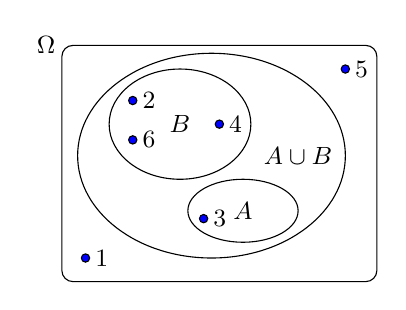
\begin{tikzpicture}[x=10mm,y=10mm,font=\small]
\def\insieme_unione{(1.9,1.6) ellipse (1.7 and 1.3)}
\def\insiemeB{(1.5,2) ellipse (.9 and .7)}
\def\insiemeA{(2.3,.9) ellipse (.7 and .4)}
\draw[rounded corners] (0,0) rectangle (4,3) (-.2,3) node {$\Omega$} ;
\draw\insieme_unione;
\draw\insiemeB node {$B$};
\draw\insiemeA node {$A$};
\draw[fill=blue] (.9,2.3)circle (1.5pt) node[right]{$2$};
\draw[fill=blue] (.9,1.8)circle (1.5pt) node[right]{$6$};
\draw[fill=blue] (2,2)circle (1.5pt) node[right]{$4$};
\draw[fill=blue] (1.8,.8)circle (1.5pt) node[right]{$3$};
\draw[fill=blue] (.3,.3)circle (1.5pt) node[right]{$1$};
\draw[fill=blue] (3.6,2.7)circle (1.5pt) node[right]{$5$};
\node at (3,1.6) {$A \cup B$};
\end{tikzpicture}
}

\newcommand{\unionecompatibili}{
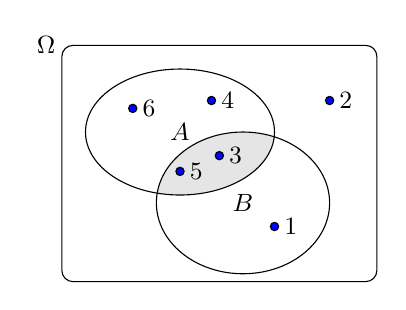
\begin{tikzpicture}[x=10mm,y=10mm,font=\small]
\def\insiemeA{(1.5,1.9) ellipse (1.2 and .8)}
\def\insiemeB{(2.3,1) ellipse (1.1 and .9)}
    \begin{scope}
        \clip \insiemeA;
        \fill[color=gray!20!] \insiemeB;
    \end{scope}
\draw[rounded corners] (0,0) rectangle (4,3) (-.2,3) node {$\Omega$} ;
\draw\insiemeB node {$B$};
\draw\insiemeA node {$A$};
\draw[fill=blue] (.9,2.2)circle (1.5pt) node[right]{$6$};
\draw[fill=blue] (3.4,2.3)circle (1.5pt) node[right]{$2$};
\draw[fill=blue] (1.9,2.3)circle (1.5pt) node[right]{$4$};
\draw[fill=blue] (2.7,.7)circle (1.5pt) node[right]{$1$};
\draw[fill=blue] (2,1.6)circle (1.5pt) node[right]{$3$};
\draw[fill=blue] (1.5,1.4)circle (1.5pt) node[right]{$5$};
\end{tikzpicture}
}

\newcommand{\eventocomplementare}{% 
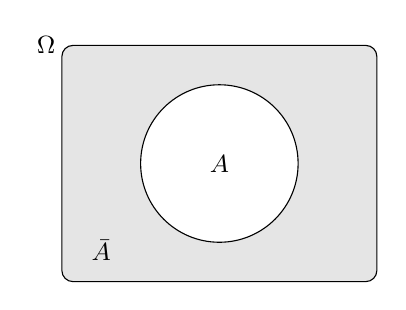
\begin{tikzpicture}[x=10mm,y=10mm,font=\small]
\definecolor{circle area}{gray}{0.9}
\draw[rounded corners, fill=circle area] (0,0) rectangle (4,3) (-.2,3) node 
{$\Omega$} ;
\node[]  at (.5,.4) {$\bar{A}$};
\draw[fill=white](2,1.5) circle (1) (2,1.5) node {$A$};
\end{tikzpicture}
}

\newcommand{\intersezioneeventi}{%
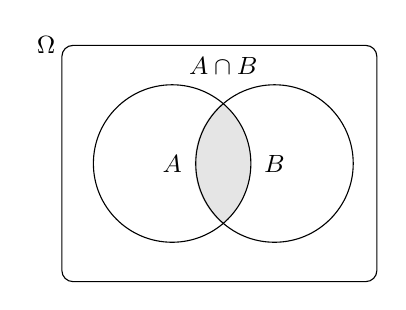
\begin{tikzpicture}[filled/.style={fill=circle area, draw=circle edge, 
thick},x=10mm,y=10mm,font=\small]
\def\firstcircle{(1.4,1.5) circle (1cm)}
\def\secondcircle{(2.7,1.5) circle (1cm)}

\definecolor{circle edge}{gray}{0.9}
\definecolor{circle area}{gray}{0.9}
    \begin{scope}
        \clip \firstcircle;
        \fill[filled] \secondcircle;
    \end{scope}
    \draw\firstcircle node {$A$};
    \draw \secondcircle node {$B$};
    \node[anchor=south] at (current bounding box.north) {$A \cap B$};
\draw[rounded corners] (0,0) rectangle (4,3) (-.2,3) node {$\Omega$} ;
\end{tikzpicture}
}

\newcommand{\prodottoeventi}{
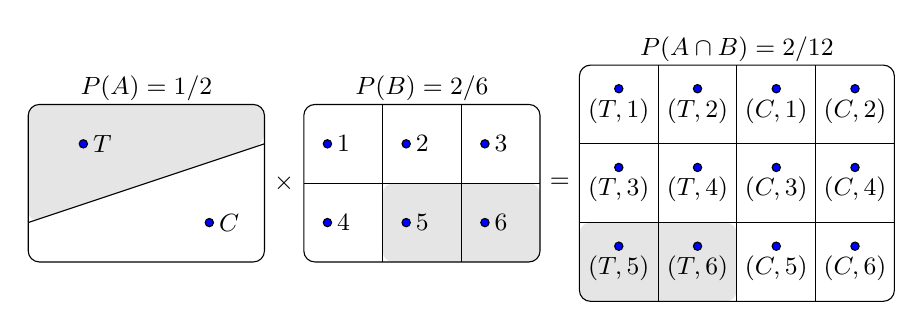
\begin{tikzpicture}[x=10mm,y=10mm,font=\small]

\def\rettangolo{-- ++(3,0) -- ++(0,2) -- ++(-3,0) -- cycle}
\def\insieme_int{-- ++(4,0) -- ++(0,3) -- ++(-4,0) -- cycle}
 %insieme1
\fill[rounded corners, color=gray!20!] 
     (0,.5) -- (0,2) -- (3,2) -- (3,1.5) -- cycle;
\draw[rounded corners] (0,0) \rettangolo;
\node at (1.5,2.2) {$P(A)=1/2$};
\draw (0,.5) -- (3,1.5);
\draw[fill=blue] (.7,1.5) circle (1.5pt) node[right] {$T$};
\draw[fill=blue] (2.3,.5) circle (1.5pt) node[right] {$C$};
%insieme 2
\fill[rounded corners, color=gray!20!] 
(4.5,0) -- (6.5,0) -- (6.5,1) -- (4.5,1) -- cycle;
\draw[rounded corners] (3.5,0) \rettangolo;
\draw (3.5,1) -- (6.5,1);
\foreach \x in {4.5,5.5}{
\draw (\x,0)--(\x,2);
\draw (\x,0)--(\x,2);}
\foreach \x in {3.8,4.8,5.8}
   \foreach \y in {0.5,1.5}
   { \draw[fill=blue] (\x,\y) circle (1.5pt);}
\draw node[right] at (3.8,1.5) {$1$};
\draw node[right] at (4.8,1.5) {$2$};
\draw node[right] at (5.8,1.5) {$3$};

\draw node[right] at (3.8,0.5) {$4$};
\draw node[right] at (4.8,0.5) {$5$};
\draw node[right] at (5.8,0.5) {$6$};
\node at (5,2.2) {$P(B)=2/6$};
\node at (3.25,1) {$\times$};
%insieme risultato
\fill[rounded corners, color=gray!20!] 
     (7, -.5) -- (9, -.5) -- (9, .5) -- (7, .5) -- cycle;
% \fill[color=gray!20!] (8,.5) -- (8,1.5) -- (9,1.5) -- (9,.5) -- cycle;
% \fill[color=gray!20!] (9,1.5) -- (9,2.5) -- (10,2.5) -- (10,1.5) -- cycle;
\draw[rounded corners] (7,-.5) \insieme_int;
\node at (9,2.7) {$P(A \cap B )=2/12$};
\node at (6.75,1) {$=$};
\foreach \x in {8,9,10}{
\draw (\x,-.5)--(\x,2.5);
\draw (\x,-.5)--(\x,2.5);
\draw (\x,-.5)--(\x,2.5);}
\foreach \y in {.5,1.5}{
\draw (7,\y)--(11,\y);
\draw (7,\y)--(11,\y);}

\foreach \x in {7.5,8.5,9.5,10.5}
   \foreach \y in {0.2,1.2,2.2}
   { \draw[fill=blue] (\x,\y) circle (1.5pt);}

\draw node[below] at (7.5,2.2) {$(T,1)$};
\draw node[below] at (8.5,2.2) {$(T,2)$};
\draw node[below] at (9.5,2.2) {$(C,1)$};
\draw node[below] at (10.5,2.2) {$(C,2)$};

\draw node[below] at (7.5,1.2) {$(T,3)$};
\draw node[below] at (8.5,1.2) {$(T,4)$};
\draw node[below] at (9.5,1.2) {$(C,3)$};
\draw node[below] at (10.5,1.2) {$(C,4)$};

\draw node[below] at (7.5,0.2) {$(T,5)$};
\draw node[below] at (8.5,0.2) {$(T,6)$};
\draw node[below] at (9.5,0.2) {$(C,5)$};
\draw node[below] at (10.5,0.2) {$(C,6)$};
\end{tikzpicture}
}

\newcommand{\alberomonetadado}{
\begin{tikzpicture}[x=10mm,y=10mm,font=\small]
\node [circle, draw] (a) {$\bullet$};
\node [circle, draw, fill=orange!20!] (t) [above right=of a] {$T$};
\node [circle, draw] (c) [below right=of a] {$C$};
\node [rectangle, draw] (d1) at(45:5.5) {$1$};
\node [right=.1 of d1]{$P(T \cap 1)=1/12$};
\node [rectangle, draw] (d2) [below =.2 of d1] {$2$};
\node [right=.1 of d2]{$P(T \cap 2)=1/12$};
\node [rectangle, draw] (d3) [below =.2 of d2] {$3$};
\node [right=.1 of d3]{$P(T \cap 3)=1/12$};
\node [rectangle, draw] (d4) [below =.2 of d3] {$4$};
\node [right=.1 of d4]{$P(T \cap 4)=1/12$};
\node [rectangle, draw, fill=orange!20!] (d5) [below =.2 of d4] {$5$};
\node [right=.1 of d5] (ad1){$P(T \cap 5)=1/12$};
\node [rectangle, draw, fill=orange!20!] (d6) [below =.2 of d5] {$6$};
\node [right=.1 of d6] (ad2){$P(T \cap 6)=1/12$};
\draw (6.7,.55) -- (7.2,.55) -- (7.2,1.2) -- (6.7,1.2);
\node at (7.4,.9) {$+$};
\node [rectangle, draw] (d11) [below =.2 of d6] {$1$};
\node [right=.1 of d11]{$P(C \cap 1)=1/12$};
\node [rectangle, draw] (d22) [below =.2 of d11] {$2$};
\node [right=.1 of d22]{$P(C \cap 2)=1/12$};
\node [rectangle, draw] (d33) [below =.2 of d22] {$3$};
\node [right=.1 of d33]{$P(C \cap 3)=1/12$};
\node [rectangle, draw] (d44) [below =.2 of d33] {$4$};
\node [right=.1 of d44]{$P(C \cap 4)=1/12$};
\node [rectangle, draw] (d55) [below =.2 of d44] {$5$};
\node [right=.1 of d55]{$P(C \cap 5)=1/12$};
\node [rectangle, draw] (d66) [below =.2 of d55] {$6$};
\node [right=.1 of d66]{$P(C \cap 6)=1/12$};

\draw[ultra thick,color=Maroon] (a) -- (t) node[midway,sloped,above] {$1/2$};
\draw (a) -- (c)node[midway,sloped,above] {$1/2$};
\draw (t) -- (d1)node[midway,sloped] {$1/6$};
\draw (t) -- (d2)node[midway,sloped] {$1/6$};
\draw (t) -- (d3)node[midway,sloped] {$1/6$};
\draw (t) -- (d4)node[midway,sloped] {$1/6$};
\draw[thick,color=Maroon] (t) -- (d5)node[midway,sloped] {$1/6$};
\draw[thick,color=Maroon] (t) -- (d6)node[midway,sloped] {$1/6$};
\draw (c) -- (d11)node[midway,sloped] {$1/6$};
\draw (c) -- (d22)node[midway,sloped] {$1/6$};
\draw (c) -- (d33)node[midway,sloped] {$1/6$};
\draw (c) -- (d44)node[midway,sloped] {$1/6$};
\draw (c) -- (d55)node[midway,sloped] {$1/6$};
\draw (c) -- (d66)node[midway,sloped] {$1/6$};

\end{tikzpicture}
}

\newcommand{\alberopalline}{
\begin{tikzpicture}[x=10mm,y=10mm,font=\small]

\filldraw[fill=gray!20!, draw=black]
(0,-1)--(0,1)--(.2,1)--(.2,-.8)--(2.3,-.8)--(2.3,1)--(2.5,1)--(2.5,-1)-- cycle;
\filldraw[fill=black, draw=black]  (.5,.5) circle (4pt);
\filldraw[fill=black, draw=black]  (1.8,-.3) circle (4pt);
\filldraw[fill=white, draw=black]  (.8,0) circle (4pt);
\filldraw[fill=white, draw=black]  (1.7,.4) circle (4pt);
\filldraw[fill=white, draw=black]  (1.2,-.5) circle (4pt);

\node [circle, draw] (a) at (5,0) {$\bullet$};
\node [circle, draw] (b1) [above right=of a] {$B_1$};
\node [circle, draw, fill=orange!20!] (n1) [below right=of a] {$N_1$};
\node [circle, draw] (b2) at(15:9) {$B_2$};
\node [right=.1 of b2] {$P(B_1 \cap B_2)=9/25$};
\node [circle, draw] (n2) [below =.7 of b2] {$N_2$};
\node [right=.1 of n2] {$P(B_1 \cap N_2)=6/25$};
\node [circle, draw] (b3) [below =.7 of n2] {$B_2$};
\node [right=.1 of b3] {$P(N_1 \cap B_2)=6/25$};
\node [circle, draw, fill=orange!20!] (n3) [below =.7 of b3] {$N_2$};
\node [right=.1 of n3] {$P(N_1 \cap N_2)=4/25$};
\draw (a) -- (b1)node[midway,sloped,above] {$3/5$};
\draw[ultra thick,color=Maroon] (a) -- (n1) node[midway,sloped,above] {$2/5$};
\draw (b1) -- (b2)node[midway,sloped,above] {$3/5$};
\draw (b1) -- (n2)node[midway,sloped,above] {$2/5$};
\draw (n1) -- (b3)node[midway,sloped,above] {$3/5$};
\draw[thick,color=Maroon] (n1) -- (n3) node[midway,sloped,above] {$2/5$};
\end{tikzpicture}
}

\begin{comment}

% fig012.pgf
% (c) 2013 Claudio Carboncini - claudio.carboncini@gmail.com
\begin{tikzpicture}[x=10mm,y=10mm,font=\small]

\filldraw[fill=gray!20!, draw=black]
(.7,-1)--(.7,1)--(.9,1)--(.9,-.8)--(3,-.8)--(3,1)--(3.2,1)--(3.2,-1)-- cycle;
\filldraw[fill=black, draw=black]  (1.2,.5) circle (4pt);
\filldraw[fill=black, draw=black]  (2.5,-.3) circle (4pt);
\filldraw[fill=white, draw=black]  (1.4,0) circle (4pt);
\filldraw[fill=white, draw=black]  (2.4,.4) circle (4pt);
\filldraw[fill=white, draw=black]  (1.9,-.5) circle (4pt);

\node [circle, draw] (a) at (5,0) {$\bullet$};
\node [circle, draw] (b1) [above right=of a] {$B_1$};
\node [circle, draw, fill=orange!20!] (n1) [below right=of a] {$N_1$};
\node [circle, draw] (b2) at(15:9) {$B_2$};
\node [right=.1 of b2] {$P(B_1 \cap B_2)=9/25$};
\node [circle, draw] (n2) [below =.7 of b2] {$N_2$};
\node [right=.1 of n2] {$P(B_1 \cap N_2)=6/25$};
\node [circle, draw] (b3) [below =.7 of n2] {$B_2$};
\node [right=.1 of b3] {$P(N_1 \cap B_2)=6/25$};
\node [circle, draw, fill=orange!20!] (n3) [below =.7 of b3] {$N_2$};
\node [right=.1 of n3] {$P(N_1 \cap N_2)=4/25$};
\draw (a) -- (b1)node[midway,sloped,above] {$3/5$};
\draw[ultra thick,color=Maroon] (a) -- (n1) node[midway,sloped,above] {$2/5$};
\draw (b1) -- (b2)node[midway,sloped,above] {$3/5$};
\draw (b1) -- (n2)node[midway,sloped,above] {$2/5$};
\draw (n1) -- (b3)node[midway,sloped,above] {$3/5$};
\draw[thick,color=Maroon] (n1) -- (n3) node[midway,sloped,above] {$2/5$};

\end{tikzpicture}

% fig013.pgf
% (c) 2013 Claudio Carboncini - claudio.carboncini@gmail.com
\begin{tikzpicture}[x=10mm,y=10mm,font=\small]
\filldraw[fill=gray!20!, draw=black]
(-1,-1)--(-1,.8)--(-.8,.8)--(-.8,-.8)--(.8,-.8)--(.8,.8)--(1,.8)--(1,-1)-- 
cycle;
\filldraw[fill=black, draw=black]  (-.5,.5) circle (4pt);
\filldraw[fill=black, draw=black]  (-.4,-.4) circle (4pt);
\filldraw[fill=white, draw=black]  (-.2,0) circle (4pt);
\filldraw[fill=white, draw=black]  (.4,.4) circle (4pt);
\filldraw[fill=white, draw=black]  (.2,-.5) circle (4pt);
\node at(0,1) {$P(N_1)=2/5$};

\filldraw[fill=gray!20!, draw=black]
(2,-1)--(2,.8)--(2.2,.8)--(2.2,-.8)--(3.8,-.8)--(3.8,.8)--(4,.8)--(4,-1)-- 
cycle;
\filldraw[fill=black, draw=black]  (2.6,-.4) circle (4pt);
\filldraw[fill=white, draw=black]  (2.8,0) circle (4pt);
\filldraw[fill=white, draw=black]  (3.4,.4) circle (4pt);
\filldraw[fill=white, draw=black]  (3.2,-.5) circle (4pt);
\node at(3,1) {$P(N_2/N_1)=1/4$};

\node [circle, draw] (a) at (5,0) {$\bullet$};
\node [circle, draw] (b1) [above right=of a] {$B_1$};
\node [circle, draw, fill=orange!20!] (n1) [below right=of a] {$N_1$};
\node [circle, draw] (b2) at(15:9) {$B_2$};
\node [right=.1 of b2] {$P(B_1 \cap B_2)=6/20$};
\node [circle, draw] (n2) [below =.7 of b2] {$N_2$};
\node [right=.1 of n2] {$P(B_1 \cap N_2)=6/20$};
\node [circle, draw] (b3) [below =.7 of n2] {$B_2$};
\node [right=.1 of b3] {$P(N_1 \cap B_2)=6/20$};
\node [circle, draw, fill=orange!20!] (n3) [below =.7 of b3] {$N_2$};
\node [right=.1 of n3] {$P(N_1 \cap N_2)=2/20$};
\draw (a) -- (b1)node[midway,sloped,above] {$3/5$};
\draw[ultra thick,color=Maroon] (a) -- (n1) node[midway,sloped,above] {$2/5$};
\draw (b1) -- (b2)node[midway,sloped,above] {$2/4$};
\draw (b1) -- (n2)node[midway,sloped,above] {$2/4$};
\draw (n1) -- (b3)node[midway,sloped,above] {$3/4$};
\draw[thick,color=Maroon] (n1) -- (n3) node[midway,sloped,above] {$1/4$};

\end{tikzpicture}

% fig014.pgf
% (c) 2013 Claudio Carboncini - claudio.carboncini@gmail.com
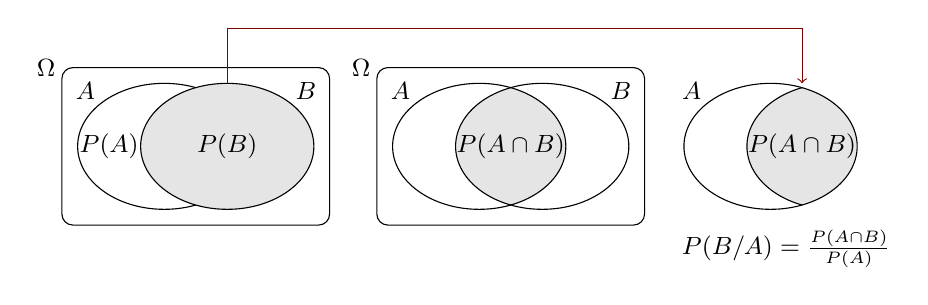
\begin{tikzpicture}[x=10mm,y=10mm,font=\small]

\def\rettangolo{-- ++(3.4,0) -- ++(0,2) -- ++(-3.4,0) -- cycle}
\def\insieme_int{-- ++(4,0) -- ++(0,3) -- ++(-4,0) -- cycle}
\def\firstcircle{(1.3,1) ellipse (1.1 and .8)}
\def\secondcircle{(2.1,1) ellipse (1.1 and .8)}
\def\thirdcircle{(5.3,1) ellipse (1.1 and .8)}
\def\fourthcircle{(6.1,1) ellipse (1.1 and .8)}
\def\fifthcircle{(9,1) ellipse (1.1 and .8)}
\def\sixthcircle{(9.8,1) ellipse (1.1 and .8)}
 %insieme1
\draw[rounded corners] (0,0) \rettangolo (-.2,2) node {$\Omega$};
\draw[->,color=Maroon] (2.1,1.8)--(2.1,2.5)--(9.4,2.5)--(9.4,1.8);
\draw \firstcircle (.6,1) node {$P(A)$} (.3,1.7) node {$A$};
\filldraw[fill=gray!20!,draw=black] \secondcircle node {$P(B)$} (3.1,1.7) 
node{$B$};

 \begin{scope}
     \clip \thirdcircle;
     \fill[color=gray!20!] \fourthcircle;
  \end{scope}

\draw \thirdcircle (4.3,1.7) node{$A$};
\draw \fourthcircle (5.7,1) node {$P(A \cap B)$}(7.1,1.7) node {$B$};
%insieme 2
\draw[rounded corners] (4,0) \rettangolo node at (3.8,2) {$\Omega$};
 \begin{scope}
     \clip \fifthcircle;
     \fill[color=gray!20!] \sixthcircle;
     \draw \sixthcircle (9.4,1) node {$P(A \cap B)$};
  \end{scope}

\draw \fifthcircle (8,1.7) node {$A$};
\draw (9.2,-.3) node {$P(B/A)=\frac{P(A \cap B)}{P(A)}$};
\end{tikzpicture}

% fig015.pgf
% (c) 2012 Dimitrios Vrettos - d.vrettos@gmail.com
\begin{tikzpicture}[x=10mm,y=10mm,font=\small]
\def\insiemeE{(2,1.5) ellipse (1.6 and 1)}
\def\firstH {(0,0)--(1.5,0)--(1,3)--(0,3)--cycle};
\def\secondH {(1.5,0)--(2.5,0)--(3,3)--(1,3)--cycle};
\def\thirdH {(2.5,0)--(4,0)--(4,3)--(3,3)--cycle};
\draw[rounded corners] (0,0) rectangle (4,3) (-.2,3) node {$\Omega$} ;
    \begin{scope}
       \clip \firstH;
       \fill[color=gray!20!] \insiemeE;
    \end{scope}
    \begin{scope}
       \clip \secondH;
       \fill[color=gray!30!] \insiemeE;
    \end{scope}
    \begin{scope}
       \clip \thirdH;
       \fill[color=gray!40!] \insiemeE;
    \end{scope}
\draw \insiemeE;
\draw(1.5,0)--(1,3);
\draw(2.5,0)--(3,3);
\draw (.5,2.7) node {$H_1$} (2,2.7) node {$H_2$} (3.5,2.7) node {$H_3$};
\draw (3.6,1.5)--(4.5,2.2) node[right]{$E$};

\begin{comment}
\draw\insiemeB node {$B$};
\draw\insiemeA node {$A$};
\draw[fill=blue] (.9,2.2)circle (1.5pt) node[right]{$6$};
\draw[fill=blue] (3.4,2.3)circle (1.5pt) node[right]{$2$};
\draw[fill=blue] (1.9,2.3)circle (1.5pt) node[right]{$4$};
\draw[fill=blue] (2.7,.7)circle (1.5pt) node[right]{$1$};
\draw[fill=blue] (2,1.6)circle (1.5pt) node[right]{$3$};
\draw[fill=blue] (1.5,1.4)circle (1.5pt) node[right]{$5$};

\end{tikzpicture}

\end{comment}
